% !TEX TS-program = latex
\documentclass[letterpaper,10pt,titlepage]{article}

\usepackage{amssymb}
\usepackage{amsmath}
\usepackage{amsthm}
\usepackage[hang,small]{caption}

\usepackage{alltt}
\usepackage{float}
\usepackage{color}
\usepackage{upquote}
\usepackage{url}

\usepackage{pstricks, pst-node}

\usepackage{geometry}
\geometry{textheight=8.5in, textwidth=6in}
\usepackage{graphicx}
%\usepackage[dvips]{graphics}
\graphicspath{{img/}}
%random comment

\newcommand{\cred}[1]{{\color{red}#1}}
\newcommand{\cblue}[1]{{\color{blue}#1}}

\usepackage{hyperref}
\usepackage{geometry}

\usepackage{listings}
\lstset{
  language=C++,
  upquote=true,
  aboveskip=3mm,
  belowskip=3mm,
  showstringspaces=false,
  columns=flexible,
  basicstyle={\small\ttfamily},
  numbers=none,
  numberstyle=\tiny\color{gray},
  keywordstyle=\color{blue},
  commentstyle=\color{dkgreen},
  stringstyle=\color{mauve},
  breaklines=true,
  breakatwhitespace=true,
  tabsize=3
}
\setlength{\parindent}{0cm}
\setlength{\parskip}{0.8em}

\captionsetup[figure]{labelfont=it,font=it}
\captionsetup[table]{labelfont={it,sc},font={it,sc}}

\def\name{Lane Breneman,Joshua Deare, Hari Caushik}
\title{Stopify - Real time road sign detection}
\date{June 12th, 2015}
\author{Lane Breneman, Joshua Deare, Hari Caushik}
\begin{document}
\maketitle
\newpage
\setcounter{tocdepth}{5}
\setcounter{secnumdepth}{5}
\tableofcontents
\newpage
\addcontentsline{toc}{section}{Introduction}
\section*{Introduction}
%Who requested it?
%Why was it requested?
%What is its importance?
%Who was your client? 
%Who are the members of your team?
%What were their roles?
%What was the role of the client(s)? (I.e., did they supervise only, or did they participate in doing development) 
Our clients, ON Semiconductor requested that we research and implement computer
vision algorithms to be able to detect street signs from video or still images
intended to be captured from a low cost camera inside an automobile. The 
algorithms were required to run on low cost development boards like the 
Beaglebone Black and the NVIDIA Jetson TK1. ON Semiconductor recently acquired
Aptina, the leading producer of CMOS image sensors and hope to enter into the
Automotive Safety industry sometime in the future. They intended this to be a 
research project in which we can research, develop and test a variety of stop 
sign detection algorithms and analyze them to determine which algorithms seem
most promising, which development boards are most promising and provide a base 
for future senior design projects to contribute to.

Our clients at ON Semiconductor were Matthew Zochert, Carl Price and Don Reid.
The members of our team were Joshua Deare, Lane Breneman and Hari Caushik. 
Throughout the year, we each contributed to the creation of the algorithm 
development framework, testing framework, capturing of images and video for 
the test dataset and presenting our work. Our clients tracked our progress,
provided suggestions for our algorithms, use of hardware, and the presentation
of our work and even provided us with starter code early on to ramp up on 
programming with the OpenCV C++ library. 
\newpage

\vspace*{\fill}
\begin{center}
\begin{minipage}{0.6\textwidth}
\addcontentsline{toc}{section}{Original Requirements Document}
\section*{Original Requirements Document}
\end{minipage}
\end{center}
\vfill

\newpage

\addcontentsline{toc}{section}{Main Project Changes}
\section*{Main Project Changes}
For the most part, our project stuck to the original specifications. The main
changes are below:

\begin{center}
    \begin{tabular}{ | l | p{5cm} | p{5cm} | p{5cm} | }
    \hline
    No. & Requirement & Changes & Reason \\ \hline
    3 & Create a database of 400 images with and without stop signs as well as
    10 videos of approaching stop signs at various speeds & Database of 173
    images was compiled & Needed to start testing algorithms and 173 was
    sufficient as a start \\ \hline
    31 & Port implementation of Algorithm 2 to Beaglebone and Jetson & 
    Algorithm 2 only ported to Jetson & Beaglebone found not to be an optimal
    platform \\ \hline
    32 & Port implementation of Algorithm 3 to Beaglebone and Jetson & 
    Algorithm 3 only ported to Jetson & Beaglebone found not to be an optimal
    platform \\ \hline
    33 & Port implementation of Algorithm 4 to Beaglebone and Jetson & 
    Algorithm 4 only ported to Jetson & Beaglebone found not to be an optimal
    platform \\ \hline
    34 & Port implementation of Algorithm 5 to Beaglebone and Jetson & 
    Algorithm 5 only ported to Jetson & Beaglebone found not to be an optimal
    platform \\ \hline
    35 & Port implementation of Algorithm 6 to Beaglebone and Jetson & 
    Algorithm 6 only ported to Jetson & Beaglebone found not to be an optimal
    platform \\ \hline
    37 & Determine the best running algorithm for use with the Beaglebone &
    Beaglebone no longer considered as an acceptable platform & Beaglebone 
    found not to be an optimal platform \\ \hline
    \end{tabular}
\end{center}

\begin{figure}[H]
    \centering
    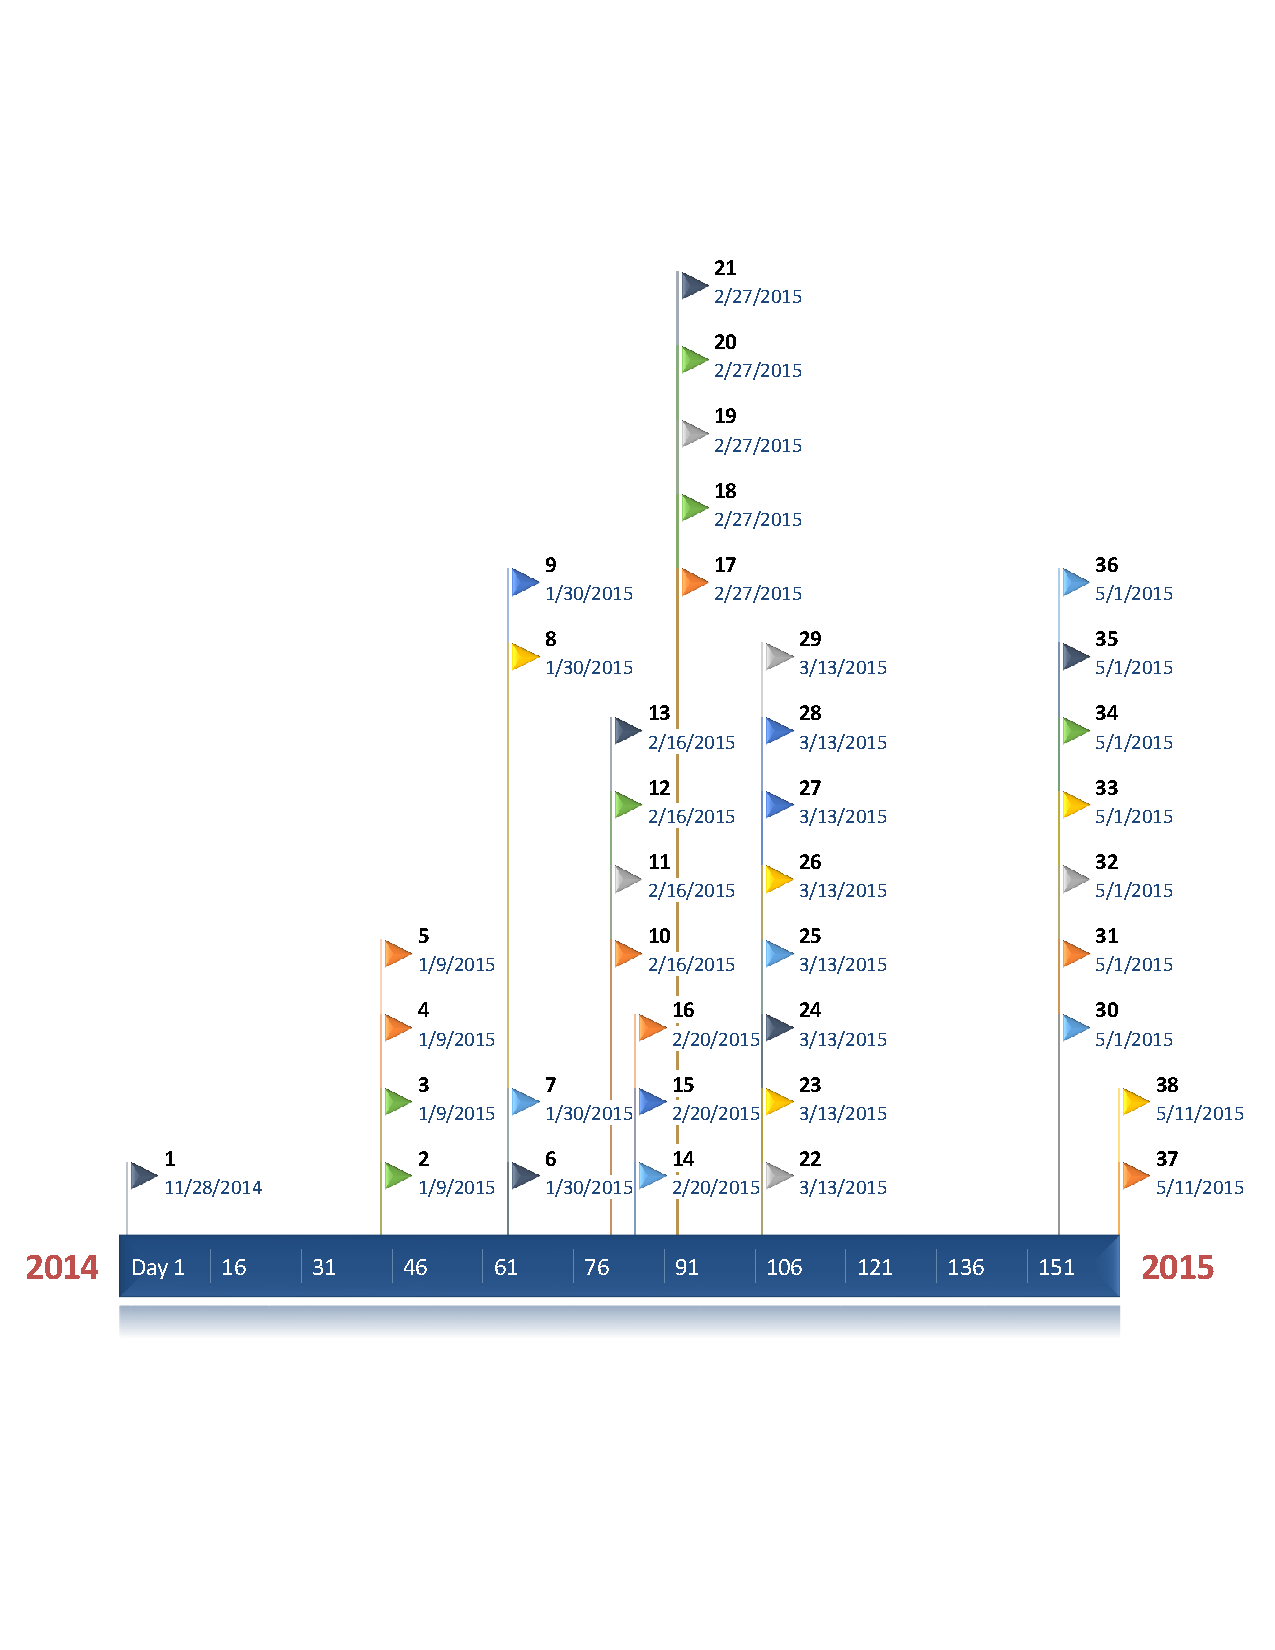
\includegraphics[width=0.8\textwidth]{ganttafter.pdf}
    \caption{Final Gantt Chart.}
\end{figure}

\addcontentsline{toc}{section}{Weekly Blog Posts}
\section*{Weekly Blog Posts}
    \paragraph*{10/31/14}
    Welcome to our first blog post for our senior capstone project. This week
    we continued our planning by evaluating the tools that we will use in order
    to complete our project. By doing this we now have a better idea of how all
    of the pieces will fit together into a final project. It also helped us to
    formalize our decision making process forcing us to look at other choices
    than just our gut feeling.

    Moving forward we will need to meet with our client and update them about 
    our software decisions and get feedback. Additionally we will be able to 
    pick up the Beaglebone Black from them meaning we can start working on the
    project!
    \paragraph*{11/7/14}
    This week, we met with our clients at Aptina and discussed and obtained 
    feedback about our technical review. In addition, we received a Beaglebone
    Black with an Aptina image sensor from them. We will begin development with
    this platform. We also clarified logistics and have set up a biweekly 
    meeting schedule. We have made arrangements to obtain a signature for our 
    requirements document. 
    \paragraph*{11/14/14}
    This week we set up our Beaglebone Black as well as our NVIDIA Shield so 
    that they are available for ssh access. This means any of us will be able 
    to work on the required hardware without us having to worry about passing
    them back and forth. 

    Additionally we took steps towards setting up our github and getting all of
    us added. 

    In the next week we will be working on getting the requirements document
    done and approved by our client.
    \paragraph*{11/21/14}
    We have completed our requirements document and now need to get it approved
    by our clients and obtain a signature from them. We plan to meet up next 
    week to do so. We are also making arrangements to obtain NVIDIA Jetson TK1 
    boards and are hoping we will get these by Winter Break so that we may be
    able to start developing on them then. 
    \paragraph*{11/28/14}
    We got our requirements document signed and approved by our clients and 
    have submitted those. We have started to think about what we would like our
    poster to look like as far as the visuals and presentation of our results.
    Also in our requirements document, we have decided on precision, recall and
    accuracy for the algorithm evaluation criteria. We are thinking about other
    such metrics.
    \paragraph*{12/5/14}
    This week we obtained an NVIDIA Jetson development board and met with our 
    client to discuss our plans for the Winter Break as well as the different
    options we have for image processing. We discussed the processing of raw 
    image file formats such as YUV as opposed to compressed file formats like 
    JPEG. Our clients also provided us with an online resource on Computer
    Vision algorithms that we will try to leverage. We created our initial 
    design for our poster and gave our elevator speech. In addition, we have 
    updated our project page with relevant documentation and have started 
    working on our final two documents for this term. 
    \paragraph*{12/12/14}
    We completed our preliminary design document and our progress report for
    this term. Our focus now shifts to developing our detection framework, 
    testing framework, and obtaining images of stop signs and not stop signs 
    for our test dataset this Winter Break. We also met with Kevin this 
    morning.
    \paragraph*{1/9/15}
    Over the Winter Break we were able to get some of the first parts of our
    project up and running. For starters we completed our framework for 
    running the different algorithms. This will allow us to start working on 
    the image detection algorithms, as well as start implementing the testing
    framework. We also wrote a tool for manually tagging the signs in images,
    this is another key component of the testing framework. The last part we 
    complete over the break was taking a ton of pictures of stop signs so once
    we have our algorithms written we will have images to test them on. 
    \paragraph*{1/16/15}
    This week we have finished our setup work and have started to work on the
    actual sign detection algorithms. We have also contacted our client and set
    up a meeting time for this term. We have aligned with each other and 
    figured out each of our specific responsibilities for completing the 
    project. For next week, we plan to continue making progress on the design,
    implementation, and testing of the sign detection algorithms. 
    \paragraph*{1/23/15}
    We have tested the detection framework and testing framework with dummy
    algorithms and both seem to work fine. We have also started to look at 
    white papers and other sources for our first algorihtms. As a starter, 
    color detection seems like a good approach and there are some sources 
    available regarding that.
    \paragraph*{1/30/15}
    This week we have continued to look at white papers for our first three 
    algorithms. There are quite a few sources available regarding street sign
    detection. We have implemented a real time color detection program with 
    the aid of the following tutorial:http://opencv-srf.blogspot.com/2010/09/object-detection-using-color-separation.html.
    We plan to use this with other machine learning algorithms. We are also 
    going to first try out these algorithms with Matlab to see if they work and
    if so, write them in OpenCV. We are also planning on having a way of 
    running each of our algorithms on every image in our testing set. 
    \paragraph*{2/6/15}
    This week, we continued implementing the street sign recognition 
    algorithms. Two of our algorithms use support vector machines and we have 
    been looking into that. One of our algorithms uses a combination of color
    detection and shape detection. The color detection is completed except for
    the inclusion of the support vector machine trained on the percentage of 
    red pixels in the training set. The shape detection also needs to be 
    added. 
    \paragraph*{2/13/15}
    We had our first checkoff in which we demoed our detection framework, 
    testing framework, test dataset, white papers, pseudocode and our first 
    algorithms. The demos went well. We now need to start thinking about our 
    next algorithms as well as porting the algorithms to the Beaglebone Black
    and Jetson as this is a non-trivial task.
    \paragraph*{2/20/15}
    We have looked at white papers for our second algorithms as well as 
    machine learning algorithms to apply to color detection. We need to start 
    implementing those soon for the final checkoff. We have also made slight 
    changes to our testing framework. 
    \paragraph*{2/27/15}
    We have three of our algorithms completed and presented those to our 
    sponsors this week. We are currently working on each of our second 
    algorithms. We are also starting to port our algorithms to the Beaglebone
    Black and Jetson, which must be completed by week 6 next term, as this can
    take a bit of time to figure out. 
    \paragraph*{3/6/15}
    We continued to work on our algorithms for the checkoff during finals week.
    We are trying to use a support vector machine along with the color 
    detection algorithm and based on a white paper also trying to combine shape
    detection with color detection for better accuracy. 
    \paragraph*{3/13/15}
    This week was spent further developing our algorithms and finalizing our 
    plans to complete the milestone by next week. We also ended up changing the
    algorithm I was working on since it was getting really poor efficiency even
    on a desktop. So instead of using a part based model, I will be attempting
    a Bag of words + svm approach that should be more efficient. Additionally
    we updated our poster with new information, although we found that until 
    our most recent algorithms are finished there was not a lot we could do.
    \paragraph*{3/20/15}
    We completed the last checkoff for this term and it went well. We have 
    ported one algorithm to the Beaglebone Black and NVIDIA Jetson and have 
    found that the Beaglebone runs way too slowly. We will need to figure out
    what we are going to do for the rest of the algorithms and whether to port 
    them to the Beaglebone or not. 
    \paragraph*{4/3/15}
    This week we continued tinkering with our algorithms and have began porting
    them to the Beaglebone and Jetson. We are also considering changing our
    requirements in light of some issues with the quality of a few of our 
    algorithms. We met with our clients and obtained feedback about our last 
    couple algorithms as well as for the Engineering Expo presentation. We are
    making plans to capture video of a car ride through Corvallis and attempt 
    to process it to demo at the Expo.
    \paragraph*{4/13/15}
    At the request of our clients, we are in the process of refining our 
    requirements to focus more on porting the implementation of our algorithms
    to the Jetson, due to the poor performance on the Beaglebone Black. We 
    were also requested to port those algorithms which were most promising to 
    the Jetson. We are in the process of selecting these also. 
    \paragraph*{4/17/15}
    We have started to port our algorithms to the Jetson. We are looking into 
    changing our code slightly for GPU acceleration. We contacted Kevin about
    our requirements changes and have received notification that they need
    to be slightly more specific. We are working on finishing that and sending
    those back into Kevin.
    \paragraph*{4/24/15}
    We have sent in our changes to our requirements and they are currently 
    being reviewed. We have ported some of our algorithms to the Jetson and are
    getting reasonable performance. We are also finding that the SVM algorithm
    with color detection is not necessarily getting good accuracy. We may need
    to stick with basic color detection or color detection coupled with shape
    detection. 
    \paragraph*{5/1/15}
    We are getting our algorithm implementations in presentable form for the 
    demo next week. We are mostly planning to run our algorithms with the 
    Jetson although we will not be able to display any graphical output. We 
    also will need to run our algorithms through the testing framework and 
    generate statistics to show in the spreadsheet as well as for the 
    compilation of results for the Engineering Expo.
    \paragraph*{5/8/15}
    We have tested our algorithms and evaluated them based on accuracy, 
    precision and recall. We are continuing to try to improve the runtime of
    our algorithms and refining them. We are continuing to work on our demo.
    We will then be in the process of organizing and documenting all of our 
    work to fulfill the requirements of this class as well as hand over to our
    clients. 
    \paragraph*{5/15/15}
    Just finished the Engineering Expo! It feels great to be done with that 
    and we are happy with the way it went. We're also exhausted!
    \paragraph*{5/22/15}
    We had our final Senior Design lecture/class this week. We have set up our
    presentation with ON employees for next Thursday. We are starting to put 
    together our presentation for that. 
    \paragraph*{5/29/15}
    We presented our project to ON employees and have started our documentation.
    We have also received our USB flash drive. We are on track to completing
    our documentation and wrapping up the project for the year. 
    \paragraph*{6/5/15}
    We are in the process of completing our documentation and our clients have
    reached out to us both to provide feedback and receive feedback on their
    mentorship. We have provided feedback to them and also have part of our 
    video done. We will meet our clients one last time next week and wrap up
    the project.

\addcontentsline{toc}{section}{Project Documentation}
\section*{Project Documentation}
% How does your project work?
% - What is its structure?
% - What is its Theory of Operation?
% - Add Block and flow diagrams
% How does one install your softare, if any?
% How does one run it?
% Are there any special hardware, OS, or runtime requirements to run your
%  software?
% Any user guides, API documentation, etc.
Our project consists of four main components: the development framework, 
algorithms, testing framework and test dataset. The development framework
provides a well defined interface to develop the computer vision algorithms and
runs the algorithms on provided images and displays the output. The algorithm 
used by the development framework is linked based on rules provided by a 
Makefile. The algorithms process the images and determine whether they contain
a stop sign or not. The testing framework is used to test the effectiveness of
each of our algorithms based on a number of evaluation metrics. It essentially
invokes the development framework and the algorithm linked to it on each image
in the test dataset.

\begin{figure}[H]
    \centering
    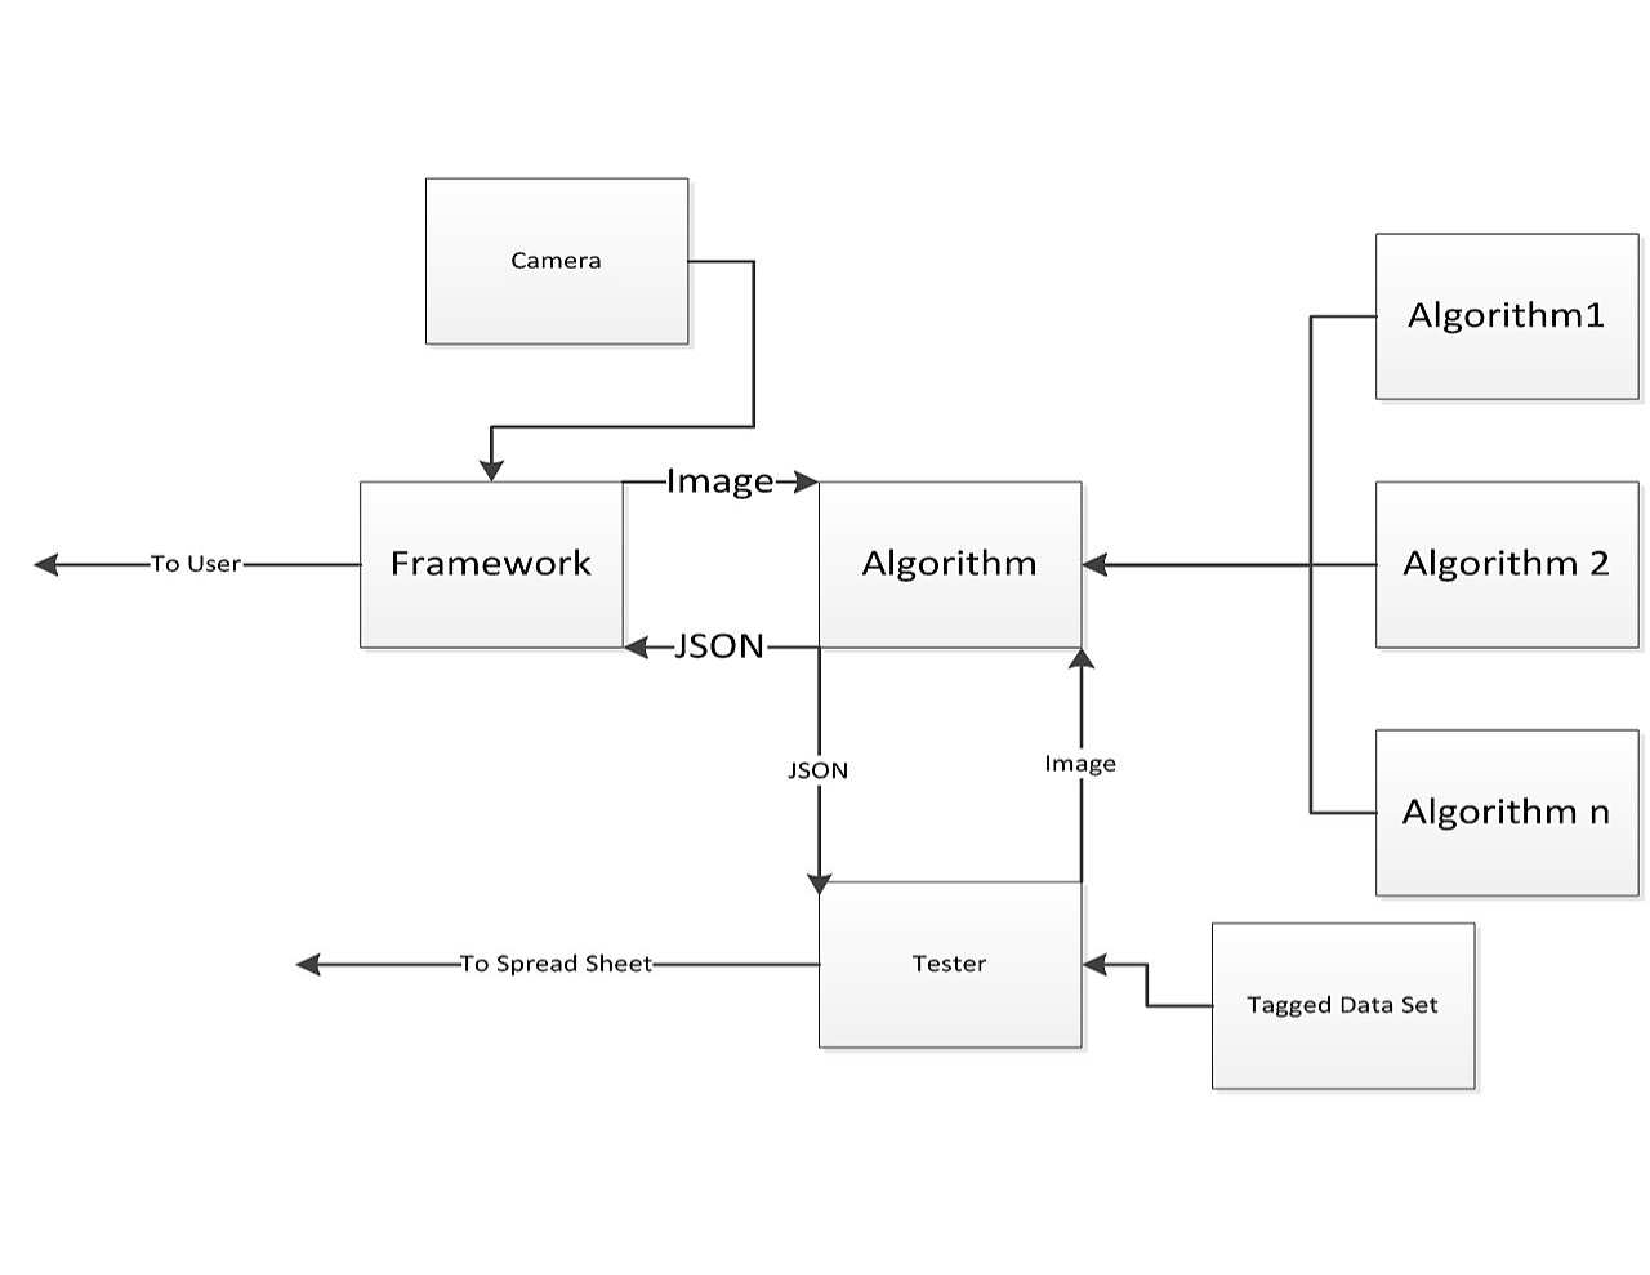
\includegraphics[width=0.8\textwidth]{dataflow.pdf}
    \caption{Basic workflow of stop sign detection.}
\end{figure}

\addcontentsline{toc}{subsection}{Development Framework}
\subsection*{Development Framework}
\paragraph*{Usage}
The development framework, written in
framework\_images/framework\_cpp/framework.cpp from the root project directory,
is a C++ program that takes a command line argument, the path of the image to
process, and returns a 1 if the algorithm determined that the image contained a
stop sign or a 0 if not. An optional third argument can be provided to display
the image being classified. For example, to classify 
framework\_images/framework\_cpp/pos\_sample.jpg, an image containing a stop
sign, the proper usage is
\begin{lstlisting}
./framework pos_sample.jpg
\end{lstlisting}
to simply return the classification result without displaying it. To display
the image, this would be
\begin{lstlisting}
./framework pos_sample.jpg 1
\end{lstlisting}
although the actual value of the third argument does not matter, just its 
presence.
\paragraph*{Implementation Details}
The development framework includes the
framework\_images/framework\_cpp/algorithm.h header file that provides the 
interface the algorithms must be written to. This is the processImage function,
with the signature
\begin{lstlisting}
int processImage(Mat &img);
\end{lstlisting}
The framework loads the test image from the path specified in the command line 
argument onto memory with the OpenCV imread function as follows:
\begin{lstlisting}
Mat img = imread(argv[1], CV_LOAD_IMAGE_COLOR);
\end{lstlisting}
The second argument specifies the loaded image to be a 3 channel color image
and the output is stored in an OpenCV Mat object, a wrapper around a 
multi-channel 2-dimensional image array.

After loading the image, the image is processed and output is displayed. If
the render option is specified, 

\begin{lstlisting}
imshow(opencvtest, img);
\end{lstlisting}

displays the image being processed.
\addcontentsline{toc}{subsection}{Algorithms}
\subsection*{Algorithms}

\addcontentsline{toc}{subsubsection}{Contour and Color Detection}
\subsubsection*{Contour and Color Detection}
\paragraph*{Description and Usage}
Contour and color detection detects stop signs by finding the contours in the
image and searching the list of contours for the characteristic octagonal 
shape of the stop sign. A contour is a curve representing the boundary of a
region in the same color. Each contour is represented by an array of points.

If the octagonal contours were found, the algorithm returns immediately as 
there is a very high probability that the image contains a stop sign. If 
however, an octagonal contour was not found, the image is then processed for 
color detection to determine the percentage of red pixels. If the percentage is
higher than a specified threshold value, the image is classified as a stop 
sign.

This algorithm is linked to the framework and run by

\begin{lstlisting}
make alg_combine
./framework [path to image file]
\end{lstlisting}

\paragraph*{Implementation Details}
The implementation of Contour and Color Detection is provided in the file 
framework\_images/framework\_cpp/alg\_combine/alg\_combine.cpp from the root 
directory of our project. The RGB image is first converted to grayscale to make
edge detection simpler by removing the extra channels with 

\begin{lstlisting}
cvtColor(Img, Img_gray, CV_BGR2GRAY);
\end{lstlisting}

The Mat object Img\_gray now contains the grayscale image. A Gaussian Blur is
then applied to this grayscale image to smooth it and remove noise. 

\begin{lstlisting}
GaussianBlur(Img_gray, Img_gray, Size(3,3), 0);;
\end{lstlisting}

The resultant image is then passed through the Canny edge detector to detect 
the edges and threshold the image. 

\begin{lstlisting}
Canny(Img_gray, canny_output, thresh, thresh*2, 3);
\end{lstlisting}

These edges are then passed into the shapeDetect function, which searches for 
the 8-sided contour. The contours are first found by the OpenCV function 
findContours.

\begin{lstlisting}
findContours(img, contour, hierarchy, CV_RETR_LIST, CV_CHAIN_APPROX_SIMPLE, Point(0,0));
\end{lstlisting}

Then the algorithm loops through each contour found and approximates a 
polygonal curve from each.

\begin{lstlisting}
approxPolyDP(contour[i], result[i], epsilon, true);
\end{lstlisting}

If the curve is 8-sided and the area enclosed is greater than a specified
amount, the image is classified as stop sign. Otherwise, if no 8-sided contours
of the minimum area were found, the algorithm passes the original image through
color detection. This is done by first converting the original Mat object to
the HSV, or hue-saturation-value color space. This allows to focus simply on 
the hue component, or the color component and ignore differences in brightness,
accounted for by the saturation and value components. This is done by

\begin{lstlisting}
cvtColor(Img, imgHSV, COLOR_BGR2HSV);
\end{lstlisting}

The HSV image is then thresholded based on a specified hue threshold.

\begin{lstlisting}
Mat imgThresholded = colorDetect(imgHSV, Scalar(iLowH, iLowS, iLowV), Scalar(iHighH, iHighS, iHighV));
\end{lstlisting}

Finally, the percentage of red is found with the getFrac function and this is
compared with a minimum percentage of red and the image is classified as a 
stop sign or not stop sign. 

\addcontentsline{toc}{subsubsection}{HOG}
\subsubsection*{HOG}
The HOG algorithm works by extracting a HOG Descriptor from a 64x128 image window
this descriptor is then run through a SVM to see whether the window contains a 
stop sign. If it does the match is added to a vector of bounding rectangles which
represent the matches. The window is then shifted over a little bit and then rerun.
This repeats until the entire image has been processed. The matches are then run 
through non-maximum suppression to eliminate overlapping matches.

To run detector code you train a model to do this navigate to the hog directory. In
the git projects this is in $/framework\_images/framework\_cpp/hog/$. From there you can
run the command(assuming you have a tagged dataset):
\begin{lstlisting}
./trainer [path to dataset json] [path to output model] -c 200 -e 1e-6 -i 450 -o .5 -s 1.10 -r 5
\end{lstlisting}
The arguments:
\begin{itemize}
    \item c - C value for the SVM (See CVSVM documentation)
    \item e - Epsilon value for the SVM (See CVSVM documentation)
    \item i - Max number of iterations while training
    \item o - Amount of overlap required to be considered a true positive
    \item s - How much the image pyramid scales when trying to match (See gpu::HOG documentation)
    \item r - How many overlapping rectangles are required during suppression to be considered a match
\end{itemize}

This will take a while but once its done it will output some basic statistics 
on how the new training set performed. To use this trained model we have to copy it
to the models folder in the root git directory. With that done edit the name of the
module files used in $detector\_server.cpp$ on line 10 like so:
\begin{lstlisting}
svm.load(<absolute path model file>); 
\end{lstlisting}


The path must be absolute since we don't know what directory $0detector\_server$ will
be run in and we want to be sure it finds the model.

With that done we can now run it, to do that you will need two terminal sessions.
In the first run:
\begin{lstlisting}
make detector_server
./detector_server 
\end{lstlisting}

In the second navigate to to the $framework\_images/framework\_cpp$ directory and run:
\begin{lstlisting}
make hog_server
make test
\end{lstlisting}
The make test isn't necessary but it will test that the server is running properly.
Now you can use it like any other algorithm in the framework.

\addcontentsline{toc}{subsubsection}{SURF and Bag of Words}
\subsubsection*{SURF and Bag of Words}
SURF and Bag of Words(BOW) are actually two algorithms that are used in conjunction to
classify an image. Classification is different than recognition in that it can't tell 
you where the stop sign is in the image, just that one exists. The algorithm works
in three stages:
\begin{enumerate}
    \item SURF is run over a tagged dataset, where it extracts the surf descriptors
        from any tags inside the image. These descriptors are added to a list.
    \item The list of all the descriptors is passed to a K-Means clustering algorithm
        that will find any groups of clustered points. These groups are then used to
        train a BOW vocabulary.
    \item We then run SURF over the full sized images in another test dataset. These
        SURF descriptors are then passed to BOW vocabulary which creates a new vector.
    \item This vector is then used to train a SVM. It is labeled positive if there is
        a tagged stop sign in the image, otherwise it is label a negative example. The
        SVM is then trained/
    \item To actually classify an image you just run 3 and 4 over an image but instead
        of training SVM you predict with it. If it predicts true there is a stop sign,
        otherwise there isn't.
\end{enumerate}

This algorithm ended up have some issues that should be kept in mind before using:
\begin{enumerate}
    \item It is slow, taking 1.5 seconds per a 400x300 image.
    \item It is only kind of accurate, the best was 72% accuracy.
    \item It is proprietary, meaning that you can't use it in any final commercial project.
        Additionally NVidia doesn't include it in the optimized OpenCV library
        which means that you will have to give up the OpenCV optimizations
        to use this algorithm on the jetson.
\end{enumerate}

To use this algorithm we first need to train it. To do this we will navigate to the
$/framework\_images/framework\_cpp/bow/$ in the git path. Once there we can run:
\begin{lstlisting}
make trainer
./trainer [taged dataset .json] [name of file to save the model to] [name of file to save vocab to]
\end{lstlisting}

You will notice that this outputs two files, the first is the SVM model, the second 
contains the vocabulary object. Both of these files should be copied to to models 
folder. Next edit detect.h and set the MODEL and VOCAB constants to be the absolute
path to the files that were just created. To run the detector you need to naviagte 
down to the $framework\_cpp$ directory. Build and run it using:
\begin{lstlisting}
make bow
make test
\end{lstlisting}

\addcontentsline{toc}{subsubsection}{Region of Interest (ROI)}
\subsubsection*{Region of Interest (ROI)}

The ROI algorithm is essentially an optimization of color/contour detection. 
But it only performs contour detection on the portion of the original image which
contains the highest concentration of red pixels. Note that the percent concentration is a static value for this ROI implementation. And must be changed based on image size.
This is certainly a shortcoming of this algorithm.
The following is the process which the algorithm works:
\begin{enumerate}
    \item Find the region which contains the most red pixels.
    \item Crop the image just to that region.
    \item Convert that crop to HSV colorspace.
    \item Perform contour detection on the HSV image.
    \item If an 8 sided convex object is detected, then we think there is a stop sign.
\end{enumerate}

To build the framework with the ROI algorithm:
\begin{lstlisting}
make roi_alg
\end{lstlisting}

Usage is simple and is of the form
\begin{lstlisting}
./roi_alg [image_name]
\end{lstlisting}

\addcontentsline{toc}{subsection}{Testing Framework}
\subsection*{Testing Framework}

The testing framework is pretty straight forward and requires two prerequisites:
\begin{enumerate}
    \item The main framework is already compiled with the algorithm you want to run
    \item You have a tagged dataset with the corresponding .json file 
\end{enumerate}
With that done to run the testing framework use:
\begin{lstlisting}
./tester [json file] [path to the result .csv you want create] [path to the framework executable]
\end{lstlisting}
This will create a .csv file with the result statistics for the algorithm.

\addcontentsline{toc}{subsection}{Test Dataset}
\subsection*{Test Dataset}
Our test dataset consisted of the following:
\begin{itemize}
    \item 2 videos recorded from a vehicle mounted camera while driving down a street well populated with stop signs
    \item 172 still images taken from vehicle's perspective, both containing and not containing stop signs.
\end{itemize}

\addcontentsline{toc}{section}{Resources}
\section*{Resources}
% What web sites were helpful (Listed in order of helpfulness)
% What, if any, reference books really helped?
% Were there any people on campus that were really helpful?
The following websites were particularly helpful:

\begin{enumerate}
    \item http://docs.opencv.org/
    We made heavy use of the OpenCV C++ documentation. It provided most of the
    functionality we needed to write our algorithms.
    \item http://stackoverflow.com/
    Stack Overflow was a great website to debug problems in our implementation
    as well as learn more about the internals of some of the OpenCV functions
    we leveraged.
    \item http://www.cse.iitd.ernet.in/~pkalra/csl783/canny.pdf
    This source provided useful information about the implementation of Canny
    Edge detection.
    \item http://opencv-srf.blogspot.com/2010/09/object-detection-using-color-seperation.html
    This is an OpenCV blog that had useful information about color detection
    and shape detection.
\end{enumerate}

In addition to these websites, we would like to give a big thank you to our 
mentors Matthew Zochert, Carl Price and Don Reid for their insights into 
stop sign recognition algorithms, hardware considerations and so much more. 

Last but not least, we would like to give a big thank you to our Senior Design
supervisor Professor Kevin McGrath and our TA throughout the year Jon Dodge for
making this project possible and for their support and insights into our 
project. 

\addcontentsline{toc}{section}{What We Learned}
\section*{What We Learned}
% What technical information did you learn?
% What non-technical information did you learn?
% What have you learned about project work?
% What have you learned about project management?
% What have you learned about working in teams?
% If you could do it all over, what would you do differently?
\addcontentsline{toc}{subsection}{Hari Caushik}
\subsection*{Hari Caushik}
By contributing to this project, I learned a fair bit of technical information. 
I improved my C++ programming skills and gained a familiarity with the OpenCV
library. In addition, I learned about the major concepts in computer vision
algorithms as well as image processing techniques. Throughout this project, I
also learned about software design practices and made practical use of
algorithmic complexity analysis.

A lot of non-technical information was also learned by doing this project. This
project required a lot of documentation at the start while we were 
determining the specifications, during the implementation when we documented 
the pseudocode and algorithmic complexity of the algorithms as well as our 
final report. My technical writing skills have improved as a result. We also 
presented our project, particularly towards the end of the year at the 
Engineering Expo to the general public, at ON Semiconductor to ON employees and
our final presentation video. 

Doing a nine month project for an actual client in industry has taught me most
of all that the main challenge is carefully defining an initially very 
loosely defined problem. Decisions that we make early on can have a very 
significant effect on the way our project may turn out. I have also learned 
that projects in the real world are very malleable. While the high level 
decisions we make early on guide our project in certain directions, specific 
requirements frequently change as we gain more knowledge through 
implementation. 

This project allowed each of use to take a project management role at different
times throughout the year. I learned most of all that establishing clear 
communication among all team members is essential to moving the project along 
smoothly. It is much easier to perform when each of us knows what is expected
of us and have clearly defined responsibilities. When this breaks down, there 
tends to be a lot of confusion and consequently inaction. 

I thoroughly enjoyed working with my team members and I feel as if things 
moved along very smoothly throughout the year. I learned how my teammates work
throughout the year and which ways I would need to adapt to make it work and
in which ways I could keep the same work habits. Overall I am very proud and 
impressed by my teammates' work and abilities and learned a lot technically
from them as well. Everyone compromised and contributed to the project. 

If I could do this project again, I would take a few more risks and attempt to
implement algorithms that were a little more advanced and would predict stop 
signs much more accurately. I wanted to ensure that we had moved the project 
forward this year. In hindsight, I think I was too conservative and wished I 
had been a little bolder.

\addcontentsline{toc}{subsection}{Lane Breneman}
\subsection*{Lane Breneman}

%What technical information did you learn?
Before this project I had used OpenCV for object recognition. That said I had
no experience working with the C++ interface and very little C++ experience in
general. Through this project I learned a lot about linking libraries, creating
make files and using classes in C++. On a different note I also learned a lot
about SVMs and machine learning. I had attempted to use these tools but had
never made much progress, but after this project I feel I have the skills to
employ them in future projects.

%What non-technical information did you learn?
I learned about taking notes and extracting the important information from 
research papers in order to reimplement their algorithms. I also learned 
how important communication between team members is. This largely came from
the fact the two of our basic algorithms turned out to be very similar and 
two of our advanced algorithms are also kind of similar. This limited the
variety of algorithms we explored, thus lowering the quality of the project.

%What have you learned about project work?
Our project integrated really nicely together, a large part of this I 
attribute to our good design. We found that we almost never needed to
fight the framework in order to get our code to run, which is nice. 
Even when last minute we need to make a way to export videos it took 
about 5 minutes to extend the framework. This reinforced the most 
import fact that I knew about project work, that a good design is 
important.

%What have you learned about project management?
Project management was a very mixed bag for our project. In the 
beginning we had very good project management, planning everything,
dividing work and communicating often. This lead to the best parts
of out project namely the framework and testing framework. Our later work
were less thought out and more divided and I feel that it can be seen in
quality of the work, as our algorithms could have been better.

%What have you learned about working in teams?
Communication is key. We had a really great group and I enjoyed working on the
project, but for most of the term the project became mostly individual. This lead
to two of our algorithms being pretty much the same. If we had communicated in 
more detail we could have seen this sooner and adapted.


%If you could do it all over, what would you do differently? 
If I could make one change I would have done 1 advanced algorithm each that we worked on over the year.
By advanced I mean more complicated than even the HOG or SURF algorithms. I feel
the project would of had more to show and been more rewarding if we had.

\addcontentsline{toc}{subsection}{Joshua Deare}
\subsection*{Joshua Deare}

%Tech knowledge
When I started this project, the only technical knowledge I had regarding the topic was 
a very brief introduction to computer vision using the Python OpenCV libraries.
Even when I had worked with these libraries before, I barely touched the surface. 
I was slightly intimidated to use C++ on this project, mostly because of the rather 
negative stigma associated with it in various places I have worked, despite having never used it myself.
I have to say I was pleasantly surprised when I realized there was not a steep learning curve,
as I have much experience in C and the object oriented parts of the language are easy enough to acclimate to from experiences in Java and Python.
In addition to learning a new language, I loved being able to dive into research papers on the topic of computer vision.
It is a fascinating topic, and one I know I'm not even close to fully understanding. 
Nonetheless, the ability to learn how a computer detects contours and harsh edges in an image has been most exhilarating.

%Non-Tech knowledge
From a non-technical perspective, I learned how to internally organize and synthesize knowledge
from a vast multitude of sources. When you are reading multiple papers and referencing tens
of websites for a project it is easy to lose track of where your sources are located.
Surprisingly to me, I found the best way for me to track technical information was
to use hard-copy documents with a color-coded highlighter and sticky note system
for organization. I learned having something tactile helps me organize my thoughts.

%Project Work
What I learned about project work was that it is crucial to have clear direction.
Our project proposal was quite vague, and I believe without having defined the
project early on that whole thing would have been a disaster. 
Thankfully, our mentors at ON were very patient and helpful in narrowing the scope
of the project such that it fit both what we as individuals wanted from senior project,
and what they wanted at ON to have completed.

%Project Management
Good management is key to success. We never explicitly declared an individual the project
manager. So throughout the project we would have one of us stepping up to make sure 
deadlines were getting met, and synthesizing all of our work for presenting. 
Unfortunately, there were times when it was unclear who was responsible for what parts of the project. 
At the times when there was more clear roles the project flourished. When leadership was confused, the project usually slowed progress.

% Teams
I have worked in teams many times for software development using many different development practices. 
However, this experience brought an unexpected twist.
I may have interpreted this incorrectly, but it seemed we were highly encouraged to organize 
our requirements such that we would rely on teammates as little as possible.
For instance, if my requirement relies on feature A to be finished, don't trust my teammate to finish feature A. Assign feature A to myself instead.
While I can understand this from the perspective of protecting one's grade, it doesn't seem to aid in team unity.
Setting our requirements so we didn't rely on one another removed incentive for communication.
I feel that the lack of communication skills was a problem for all of us. 
That being said, having non-dependent requirements probably helped in how modular our project became - something I feel was a very big plus.

% Change
If I were to do it over again I would change 2 things: better communication, and improving our test dataset.
The communication was lacking many times throughout the project, and I feel we could have
produced a more superior product had that been fixed. Also, because our dataset was fairly limited and biased, it was difficult to test our algorithms effectively.

\newpage

\vspace*{\fill}
\begin{center}
\begin{minipage}{0.6\textwidth}
\addcontentsline{toc}{section}{Appendix 1: Essential Code Listings}
\section*{Appendix 1: Essential Code Listings}
\end{minipage}
\end{center}
\vfill

\newpage
\subsection*{Detection Framework(framework\_images/framework\_cpp/framework.cpp)}
\begin{lstlisting}
/*
* Framework for testing image processing algorithms with simple C++ interface
* Last Modified: 1/11/15
*/
#include <opencv2/highgui/highgui.hpp>
#include <iostream>
#include "algorithm.h"	// interface for image processing algorithms

//#define RENDER		// define if you want to display image

using namespace cv;
using namespace std;

/*
int processImage(Mat Img) {
	int sign = 0;

	// do some processing
	return sign;
}*/

int main(int argc, char *argv[]) {
    if (argc < 2) {
	cout << "Usage: framework image_file" << endl;
	exit(EXIT_FAILURE);
    }
    int render = 0;
    int sign = 0;
#ifndef RENDER
    if(argc == 3){
	render = 1;
    }
#else
    render = 1;
#endif
    // load image data  
    Mat img = imread(argv[1], CV_LOAD_IMAGE_COLOR);

    // perform sign recognition
    sign = processImage(img);
    
    // display image/
    if(render){
	// show results of sign recognition algorithm
	sign ? cout << "This is a stop sign.\n" << endl : cout << "This is not a stop sign.\n" << endl;
	imshow("opencvtest", img);
	waitKey(0);
    }
    return sign;
}

\end{lstlisting}
\subsection*{Testing Framework(testing/tester.cpp)}
\begin{lstlisting}
#include "tester.h"
using namespace std;

int main(int argc, char**argv){
    if(argc < 3){
        cout << "Usage Format: ./tester [path to json file] [csv file to save results to] [path to executable]" << endl;
        return 0;
    }
    
    DsReader *dataset = new DsReader(argv[1]);
    if(!dataset->data_exists()){
        cout << "Error: " << argv[1] << " doesn't exist! Cannot test without a dataset." << endl;
    }

    ofstream myfile;
    myfile.open (argv[2], ios::out | ios::trunc);


    struct DsImage img_data;

    int pos_matches = 0;
    int neg_matches = 0;
    int fp = 0;
    int fn = 0;
    int tp = 0;
    int tn = 0;
    int total_p = 0;
    int total_n = 0;
    double total_exec_time = 0.0;
    int cur = 0;
    myfile << "Run Time" << "," << "Got" << "," << "Should be" << endl;
    while(dataset->has_next()){
        dataset->next(img_data);
        cur++;
        struct timespec start, finish;
        double delta_t;
        //start clock
        clock_gettime(CLOCK_MONOTONIC, &start); 
        unsigned int status = 0;
        //fork and get status
        int pid = fork();
        if(pid == 0){
            execl(argv[3], argv[3], img_data.path, NULL); 
        }else if(pid < 0){
            cout << "error: could not fork" << endl;
            return 0;
        }
        //wait for the child to stop
        wait(&status);
        //end clock
        clock_gettime(CLOCK_MONOTONIC, &finish);
        //add clock cycles taken to running total
        delta_t = (finish.tv_sec - start.tv_sec);
        delta_t += (finish.tv_nsec - start.tv_nsec) / 1000000000.0;

        total_exec_time += delta_t;
        int ispos = 0;
        //foreach tag if tag.class == "stopsign"
        for(int i=0; i < img_data.tags.size(); ++i){
            string cls = dataset->get_class(img_data.tags[i].clss);
            if(cls == "stopsign"){
                ispos = 1;
            }
        }
        if(ispos){
	    total_p++;
	}else{
	    total_n++;
	}
        if((ispos && status) || !(ispos || status)){
            pos_matches++;
            if(ispos){
		tp++;
	    }else{
		tn++;
	    }
        }else{
            if(!ispos){
		fp++;
	    }else{
		fn++;
	    }
            neg_matches++;
        }
        cout << "Testing with image " << cur << " Expected:" << (ispos? "pos" : "neg")
            << " Got:" << (status? "pos" : "neg") << endl;
        myfile << delta_t << "," << status  << "," << ispos << endl;
    }
    myfile << "Number of Samples" << "," << "Total run time(seconds)" << "," 
        << "average time per image(seconds)" << "," 
        << "total correct" << "," << "%" << ","
        << "total true positives" << "," << "% of positive images correct" << ","
        << "total true negatives" << "," << "% of negative images correct" << ","
        << "total false positive" << "," << "% of negative images misclassified" << "," 
        << "total false negative" << "," << "% of positive images misclassified" << ","
	<< "Recall" << "," << "Precision" << ","
        << endl;
    myfile << cur << "," << total_exec_time << "," 
        << (total_exec_time/cur) << "," 
        << pos_matches << "," << (((float)pos_matches)/cur)*100 << ","
        << tp  << "," << (((float)tp)/total_p)*100  << ","
        << tn << "," << (((float)tn)/total_n)*100 << ","
        << fp << "," << (((float)fp)/total_n)*100 << "," 
        << fn << "," << (((float)fn)/total_p)*100 << ","
	<< (((float)tp)/(tp+fn)) << ","
	<< (((float)tp)/(fp+tp)) << ","
	<< endl; 
}
\end{lstlisting}
\subsection*{Detection Framework Makefile(framework\_images/framework\_cpp/Makefile)}
\begin{lstlisting}
detect_includes=hog/includes/LinearSVM.o hog/includes/SampleDetector.o hog/includes/helper.o 
opencv=`pkg-config --cflags --libs opencv`
cuda=-L /usr/local/cuda/lib/

default: alg.o framework


bow/detect.o: bow/detect.cpp
	g++ -g -std=c++11 -c -o bow/detect.o bow/detect.cpp

hog/detector_client.o: hog/detector_client.cpp
	g++ -g -std=c++11 -c -o hog/detector_client.o hog/detector_client.cpp


hog/detect.o: hog/detector.cpp
	g++ -g -std=c++11 -c -o hog/detect.o hog/detector.cpp

bow: bow/detect.o framework.o
	g++ -g -c -o framework.o framework.cpp 
	g++ -g framework.o bow/detect.o -Wall -o framework $(opencv)

hog: hog/detect.o framework.o
	g++ -g -c -o framework.o framework.cpp 
	g++ -g framework.o hog/detect.o $(detect_includes) -Wall -o framework $(opencv) $(cuda)

hog_server: hog/detector_client.o
	g++ -g -c -o framework.o framework.cpp
	g++ -g framework.o hog/detector_client.o $(detect_includes) -Wall -o framework $(opencv) $(cuda)


hog_demo_realtime: hog/detector_client.o
	g++ -g -c -o demo_realtime.o demo_realtime.cpp
	g++ -g demo_realtime.o hog/detector_client.o $(detect_includes) -Wall -o demo_realtime $(opencv) $(cuda)

hog_demo_preproc: hog/detector_client.o
	g++ -g -c -o demo_preproc.o demo_preproc.cpp
	g++ -g demo_preproc.o hog/detector_client.o $(detect_includes) -Wall -o demo_preproc $(opencv) $(cuda)

hog_demo_run: hog_demo_realtime hog_demo_preproc 
	#./demo_realtime test_videos/Stop1.mp4 demo_videos/hog_demo_realtime.mpg 
	#./demo_realtime test_videos/Stop2.mp4 demo_videos/hog_demo_realtime2.mpg 
	./demo_preproc test_videos/Stop1.mp4 demo_videos/hog_demo_preproc.mpg 
	./demo_preproc test_videos/Stop2.mp4 demo_videos/hog_demo_preproc2.mpg 

alg_combine_demo_realtime: alg_combine/alg_combine.o
	g++ -g -c -o demo_realtime.o demo_realtime.cpp
	g++ -g demo_realtime.o alg_combine/alg_combine.o $(detect_includes) -Wall -o demo_realtime_combine $(opencv) $(cuda)

alg_combine_demo_preproc: alg_combine/alg_combine.o
	g++ -g -c -o demo_preproc.o demo_preproc.cpp
	g++ -g demo_preproc.o alg_combine/alg_combine.o $(detect_includes) -Wall -o demo_preproc_combine $(opencv) $(cuda)

alg_combine_demo_run: alg_combine_demo_realtime alg_combine_demo_preproc 
	./demo_realtime_combine test_videos/Stop1.mp4 demo_videos/alg_combine_demo_realtime.mpg 
	./demo_realtime_combine test_videos/Stop2.mp4 demo_videos/alg_combine_demo_realtime2.mpg 
	./demo_preproc_combine test_videos/Stop2.mp4 demo_videos/alg_combine_demo_preproc.mpg 
	./demo_preproc_combine test_videos/Stop2.mp4 demo_videos/alg_combine_demo_preproc2.mpg 

roi/alg2.o: roi/alg2.cpp
	g++ -g -c -o roi/alg2.o roi/alg2.cpp

roi_demo_realtime: roi/alg2.o
	g++ -g -c -o demo_realtime.o demo_realtime.cpp
	g++ -g demo_realtime.o roi/alg2.o -Wall -o demo_realtime_roi $(opencv) $(cuda)

roi_demo_preproc: roi/alg2.o
	g++ -g -c -o demo_preproc.o demo_preproc.cpp
	g++ -g demo_preproc.o roi/alg2.o -Wall -o demo_preproc_roi $(opencv) $(cuda)

roi_demo_run: roi_demo_realtime roi_demo_preproc 
	./demo_realtime_roi test_videos/Stop1.mp4 demo_videos/roi_demo_realtime.mpg 
	./demo_realtime_roi test_videos/Stop2.mp4 demo_videos/roi_demo_realtime2.mpg 
	./demo_preproc_roi test_videos/Stop1.mp4 demo_videos/roi_demo_preproc.mpg 
	./demo_preproc_roi test_videos/Stop2.mp4 demo_videos/roi_demo_preproc2.mpg 

test: hog_server
	-./framework pos_sample.jpg 
	-./framework neg_sample.jpg

framework: alg.o algorithm.h framework.cpp 
	g++ -g alg.o -o framework framework.cpp $(opencv)

alg.o:	alg.cpp algorithm.h
	g++ `pkg-config --cflags opencv` -g -c alg.cpp  

alg_combine.o:	alg_combine/alg_combine.cpp 
	g++ -g -std=c++11 -c -o alg_combine/alg_combine.o alg_combine/alg_combine.cpp

alg_combine: alg_combine.o framework.o
	g++ -g -c -o framework.o framework.cpp
	g++ -g framework.o alg_combine/alg_combine.o -Wall -o framework $(opencv) $(cuda)

demo_realtime: alg.o demo_realtime.cpp
	g++ -g alg.o demo_realtime.cpp -Wall -o demo_realtime $(opencv) $(cuda)

clean:
	rm -f framework framework_exec dummyalg alg.o

\end{lstlisting}
\newpage

\vspace*{\fill}
\begin{center}
\begin{minipage}{0.6\textwidth}
\addcontentsline{toc}{section}{Appendix 2: Other Material}
\section*{Appendix 2: Other Material}
\end{minipage}
\end{center}
\vfill

\newpage
\begin{figure}[H]
    \centering
    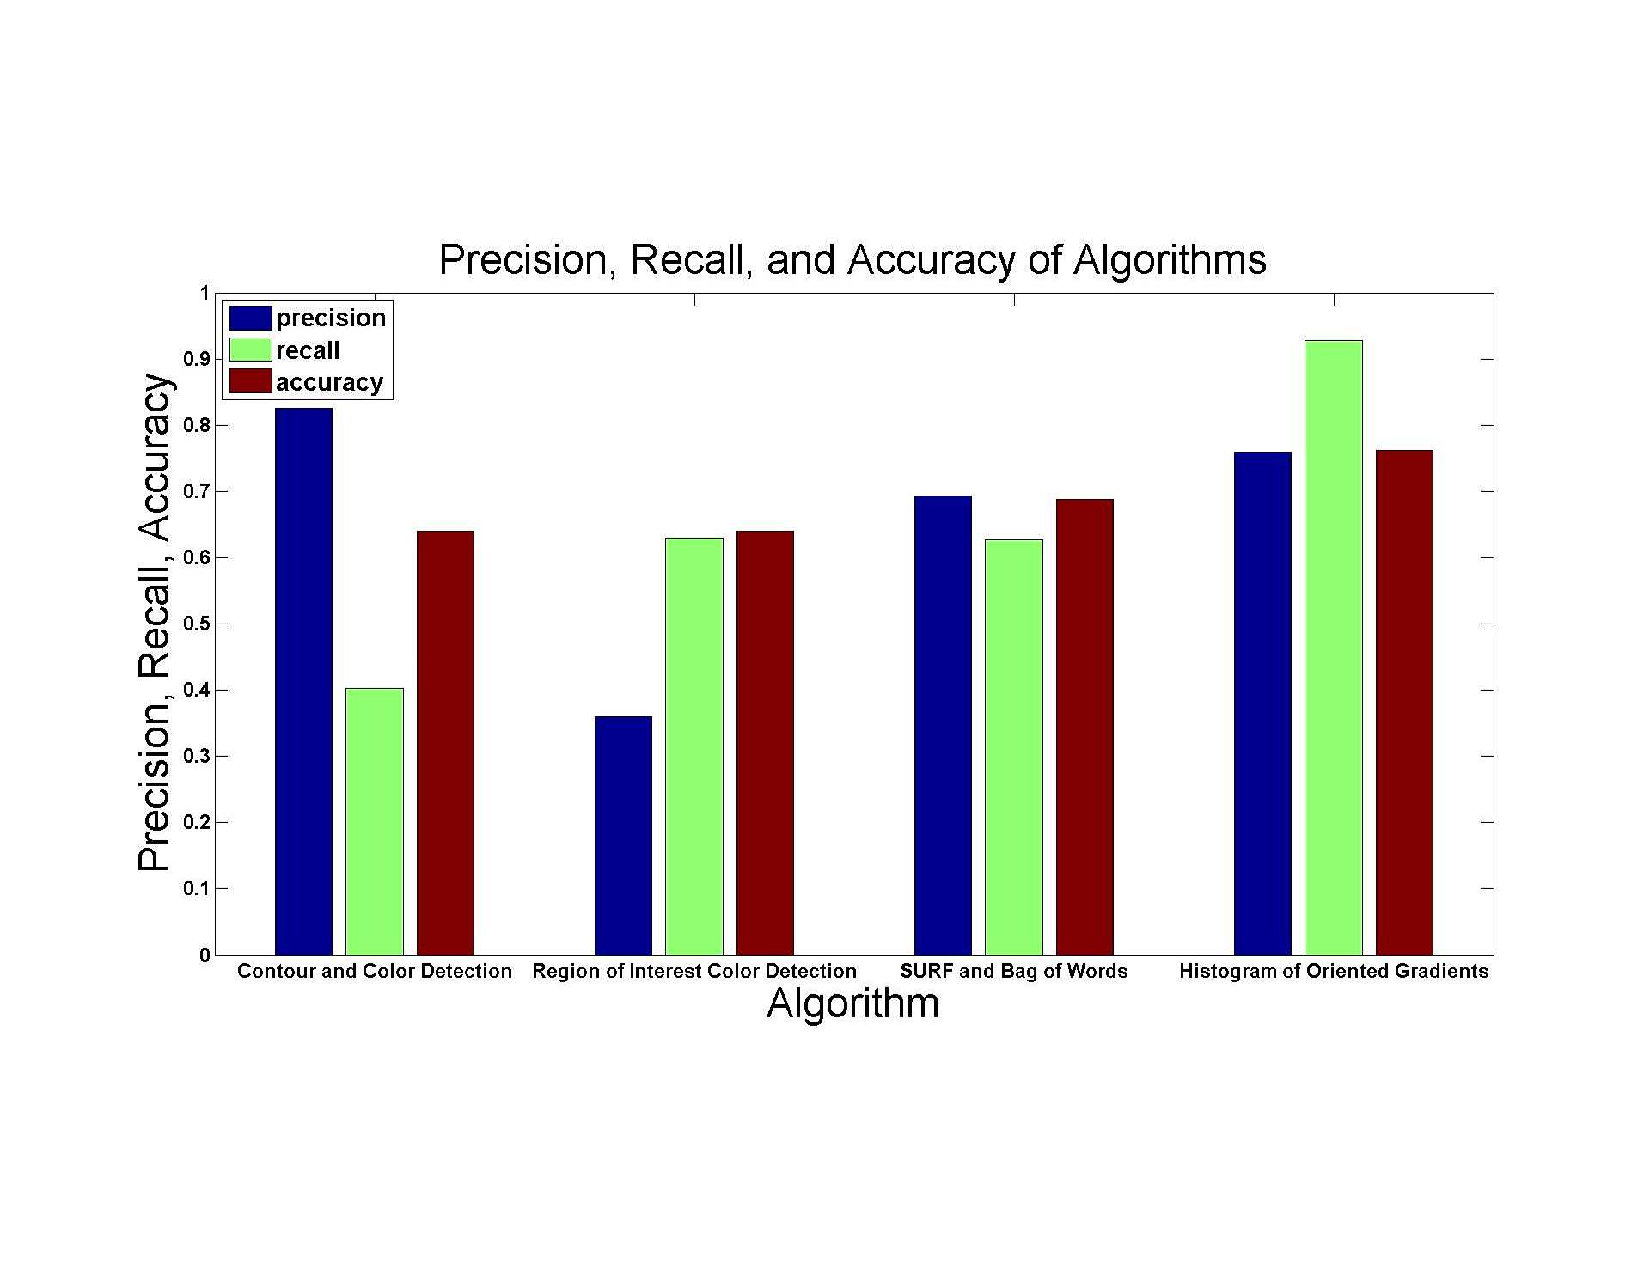
\includegraphics[width=0.8\textwidth]{alg_eval.pdf}
    \caption{Accuracy, Precision and Recall of the four best algorithms.}
\end{figure}

\begin{figure}[H]
    \centering
    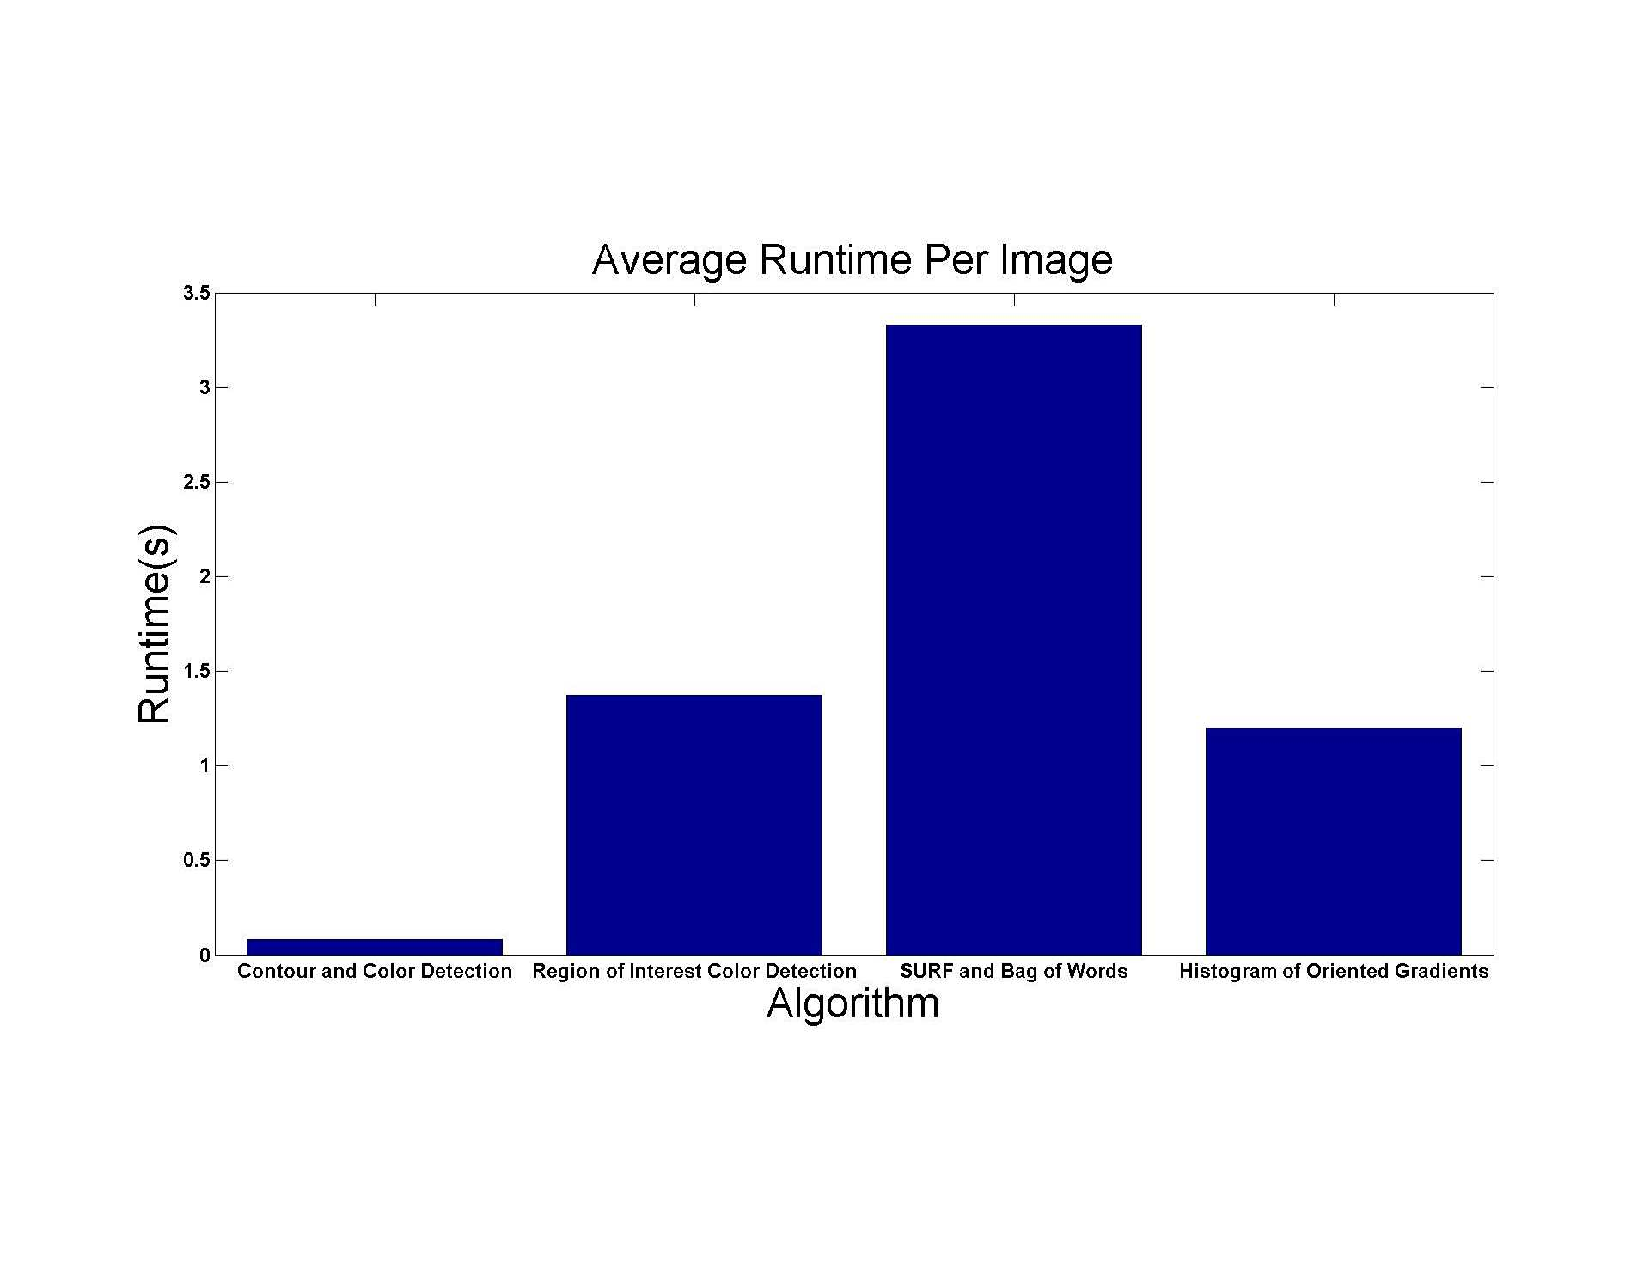
\includegraphics[width=0.8\textwidth]{runtime.pdf}
    \caption{Runtime of the four best algorithms}
\end{figure}

\end{document}
